%! TEX root = /home/duy/TUB/Thesis/latex-source/DiplomarbeitLaTex.tex

\chapter{Evaluation\label{cha:evaluation}}
In this chapter we describe how we evaluate the data generated from GAN using a baseline
classifier. The basic idea is to implement a baseline Machine Learning task and compare
the task's performances between using real data and using data generated from GAN.
Different levels of noise injection are also used in order to evaluate how the
baseline task uses depth and RGB information to make decisions.


\section{Baseline performance on original data}
In the first experiment, we try to reproduce the paper results \todo{cite eitel}. We train
a deep classifier in the following settings:

\begin{itemize}
		\item Using the original data with both Depth and RGB information
		\item Using only a part of the original data (in different scales) with both Depth and RGB information
		\item Using a part of the data (in different scales) with both Depth and RGB
			information, the remaining is substituted
			by GAN generated data
		\item Using the original data but with only RGB information in different scales,
			which is to determine the contribution that Depth data adds to the learning
			procedure
\end{itemize}

The results is reported in figure \ref{fig:eitel_accuracies}.

\begin{figure}[h]
	\caption{Classification accuracies on Washington Dataset}
	\centering
	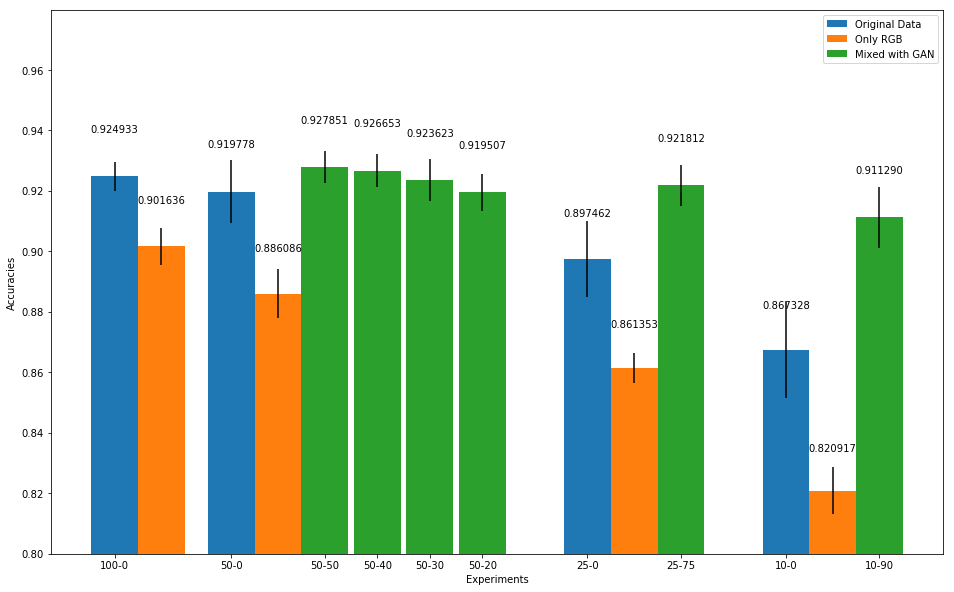
\includegraphics[width=0.75\textwidth]{img/eitel_accuracies}
	\label{fig:eitel_accuracies}
\end{figure}

\begin{figure}[h]
	\centering
	\begin{subfigure}{0.49\textwidth}
		\centering
		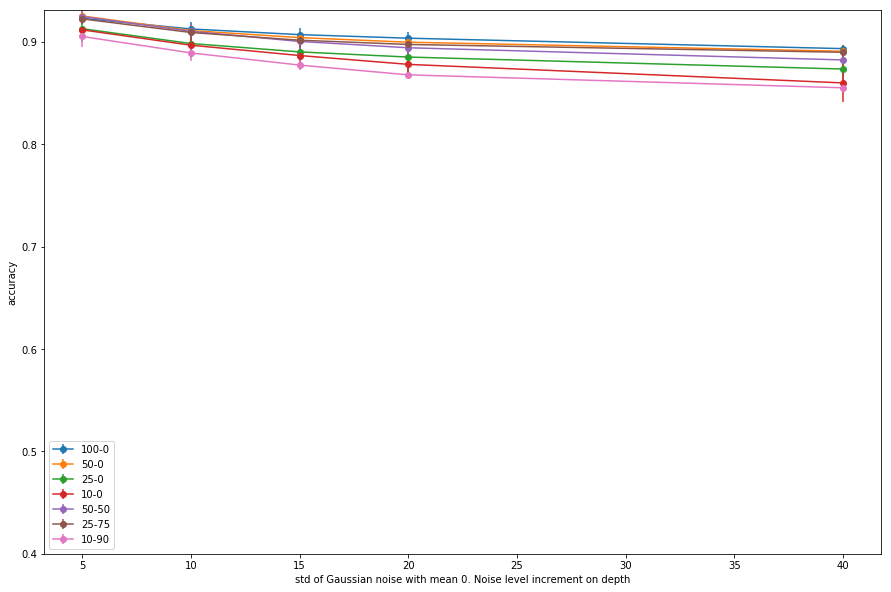
\includegraphics[width=\textwidth]{img/noise_injection_depth}
		\caption{Adding noises to depth}
	\end{subfigure}
	\begin{subfigure}{0.49\textwidth}
		\centering
		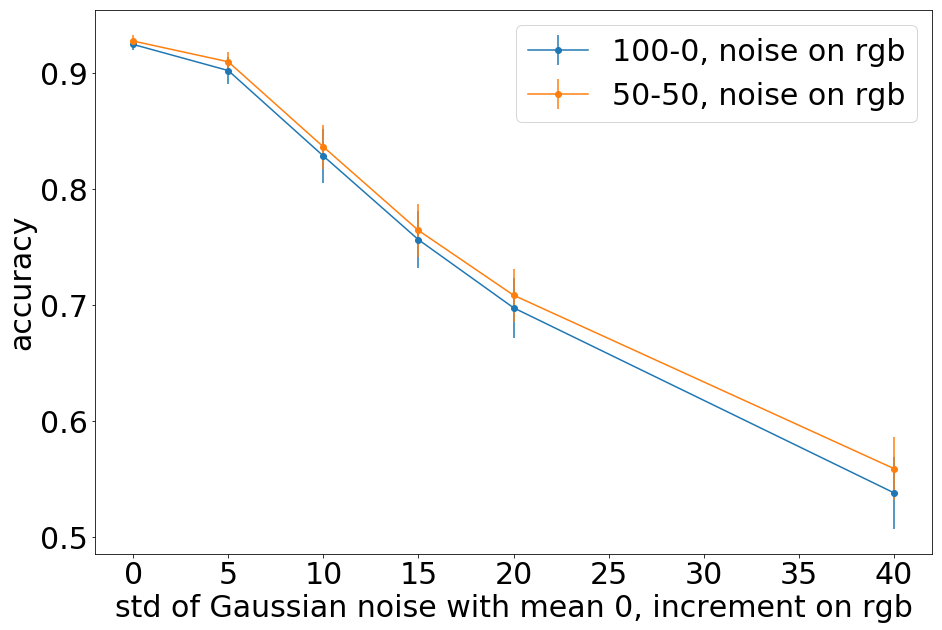
\includegraphics[width=\textwidth]{img/noise_injection_rgb}
		\caption{Adding noises to RGB}
	\end{subfigure}
	\caption{Noise Injection experiment}
	\label{fig:noise_injection}
\end{figure}

\section{Baseline performance on half of the data}
\subsection{Pure original data, without GAN data}
\subsection{With GAN data}
\section{Baseline performance on a quarter of the data}
\subsection{Pure original data, without GAN data}
\subsection{With GAN data}
\section{Baseline performance on 10\% of the data}
\subsection{Pure original data, without GAN data}
\subsection{With GAN data}
